\section{Implementación de {TRNG} basado en {RO}s}

En este Capítulo se estudia el uso de los {RO}s como generadores de números aleatorios ({TRNG}).
Se explica el diseño, hecho para {ALTERA Cyclone} III, usando primitivas de bajo nivel.
Se consideran dos características relevantes de un {RNG} para validar el diseño: 1) ll equiprobabilidad de todos los resultados posibles y 2) la estadística independencia de valores consecutivos.
En este trabajo, estas propiedades se miden a través de Cuantificadores de teoría de la información descriptos en la Sección \ref{sec:ITQs}.
Se utiliza el plano de doble entropía para representar las series de tiempo y visualizar fácilmente los resultados obtenidos con diferentes configuraciones.
La calidad estadística también se compara con otros {RNG} disponibles por medio de este plano.
Nuestro método constituye una reducción efectiva del análisis completo realizado con test estadísticos estándar como {DIEHARD} o {NIST}.

\subsection{Introducción}
\label{sec:IntroROTRNG}

Como se dijo en la Sección anterior, el jitter y los ruidos de fase presentes en los osciladores en anillo no son convenientes en muchas aplicaciones de {RO}s, por ejemplo en la implementación de {osciladores en el chip} para generar relojes en circuitos de alta velocidad \cite{Hajimiri1999, Mandal2010, Gupta2011}.
Sin embargo, son la fuente de aleatoriedad para un {TRNG} basado en {RO}s \cite{Sunar2007, Wold2009}.
Además, un {RO} se puede implementar en un circuito totalmente digital como {FPGA}s ya que básicamente son solo una serie de inversores.

En \cite{Sunar2007}, Sunar et al. presentaron un {RNG} usando \textit{jitter} estocástico combinando varios {RO}s.
Ellos requerían un procesamiento posterior del flujo de bits, para enmascarar imperfecciones en la fuente de entropía y para aumentar la inmunidad contra los cambios en las condiciones ambientales.

Wold et al. \cite{Wold2009} propusieron una versión con mejores características aleatorias y que no requieren un procesamiento posterior.
Ellos sólo agregaron un flip-flop D adicional en cada salida de anillo.
La efectividad de su propuesta fue probada por medio de pruebas estadísticas disponibles en la literatura abierta \cite{NIST2000, Marsaglia1995, NIST2000a}.

En este Capítulo se realiza una descripción detallada de una implementación de hardware muy compacta de {TRNG}s basados en {RO}s propuesto en \cite{Wold2009}.
Para validar la aleatoriedad de las secuencias de ruido generadas, se emplearon dos cuantificadores derivados de la teoría de la información y el plano de doble entropía $H_{BP} \times H_{hist}$ propuestos en la Sección \ref{capCuanti}.
Según lo explicado arriba, $H_{hist}$ es una medida de la equiprobabilidad entre todos los valores posibles y $H_{BP}$ es una medida de la independencia entre valores consecutivos.

\subsection{Implementación en Hardware}

Los {TRNG} implementados consisten en varios {RO}s con sus salidas XOR conectadas y muestreadas por un flip-flop \emph{D}.
El flip-flop latchea la salida a una frecuencia seleccionada (aquí $ 100 $ MHz) \cite{Wold2009}.
La implementación física se realizó en el kit de desarrollo {EP3C120F780C7N} {FPGA} cuyo dispositivo principal es una  {ALTERA} {Cyclone} III {EP3C120}.
El diseño está hecho con el software {Quartus} II 13.1.

\subsubsection{Reseña del Chip}

Las {FPGA}s consisten en una gran cantidad de bloques de matriz lógica ({LAB}s), con grupos de elementos lógicos ({LE}s) para implementar circuitos tanto secuenciales como combinacionales.
En la arquitectura de la familia {Cyclone} III cada {LAB} contiene $16$ {LE}s.
Básicamente, cada {LE} consiste en un flip-flop ({FF}) con una Look up table ({LUT}) de cuatro entradas (ver Figura \ref{fig:LE}).
Cada {LUT} puede implementar cualquier función de cuatro variables.
El {FF} y la {LUT} se pueden usar juntos o independientemente, \cite{Altera}.
%
\begin{figure}
\begin{center}
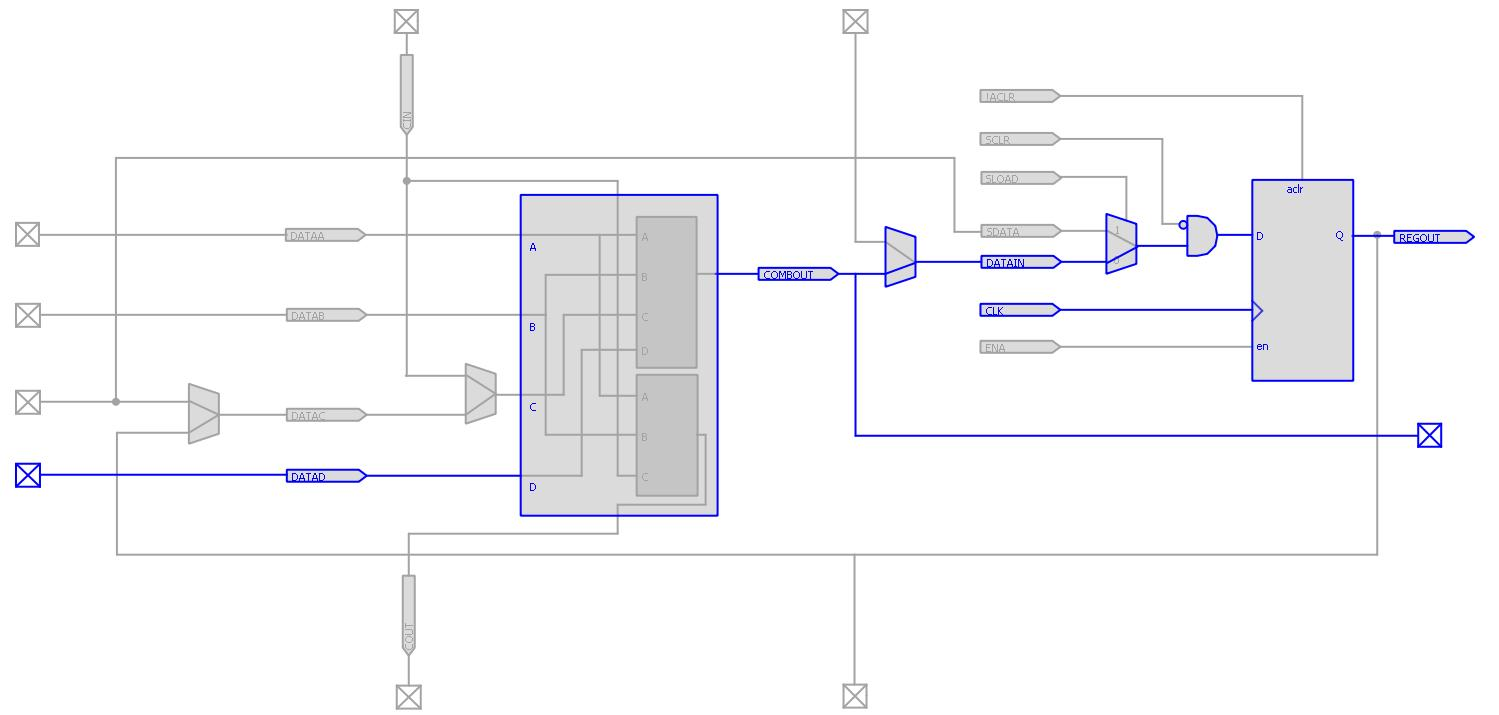
\includegraphics[ width=0.5\textwidth]{NOTenLEmasFF}
\caption{Imagen del Chip Planner que muestra la implementación de un inversor y un Flip Flop.} \label{fig:LE}
\end{center}
\end{figure}

Por lo general, el software de síntesis asigna recursos sin la intervención del diseñador.
Pero en el diseño de {TRNG}s basados en {RO}s es necesario controlar la ubicación exacta de cada componente individual  para evitar la simplificación de los inversores realizada por la herramienta de síntesis.
En {Altera} el uso de primitivas de bajo nivel permite controlar la implementación.
Por consiguiente, estas primitivas y asignaciones de bajo nivel se emplean dentro del código {HDL} empleado en el diseño desarrollado.
Además, se debe configurar la herramienta de síntesis para evitar que elimine los búferes redundantes.

Las cadenas de {RO}s se pueden implementar en el chip programando las {LUT}s como inversores.
Es necesario evitar que el motor de síntesis {Quartus} II fusione dos compuertas {NOT} en serie, utilizando una primitiva llamada {LCELL}.
Una {LCELL} consume una celda lógica y no es eliminada del proyecto durante la síntesis lógica.
Para crear un {RO}, se programan {LCELL}s como búferes de inversores.
Las Figuras \ref{fig:RTL1ring} y \ref{fig:postMap1ring} muestran como esta primitiva es implementada por el compilador Quartus II.
%
\begin{figure*}
\begin{center}
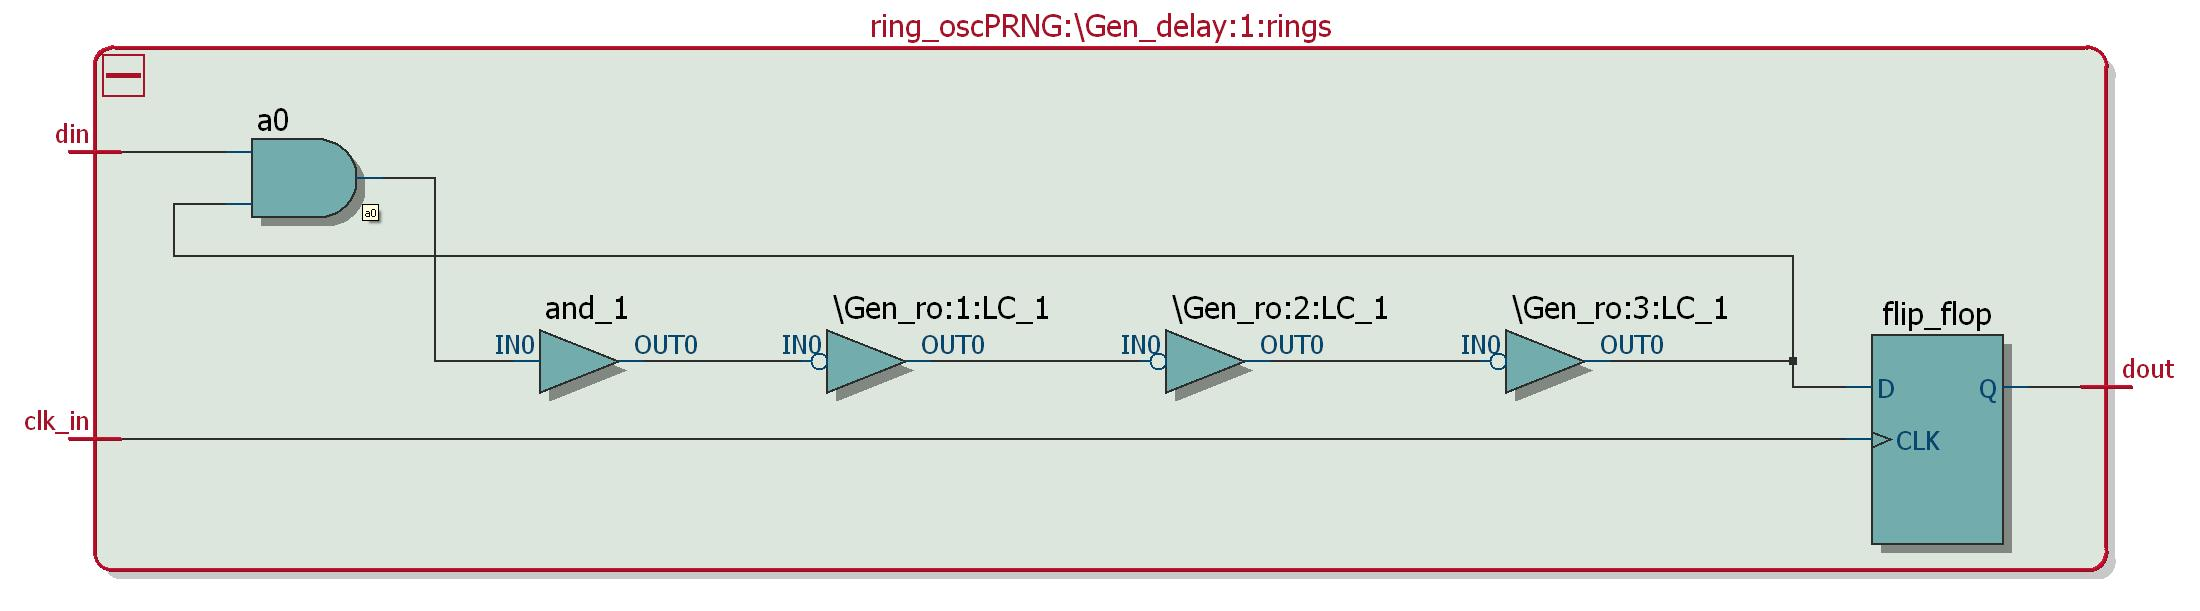
\includegraphics[width=0.7\textwidth]{RTL_view_1ring}
\caption{Vista RTL de un ring con $3$ inversores.}
\label{fig:RTL1ring}
\end{center}
\end{figure*}
%
\begin{figure*}
\begin{center}
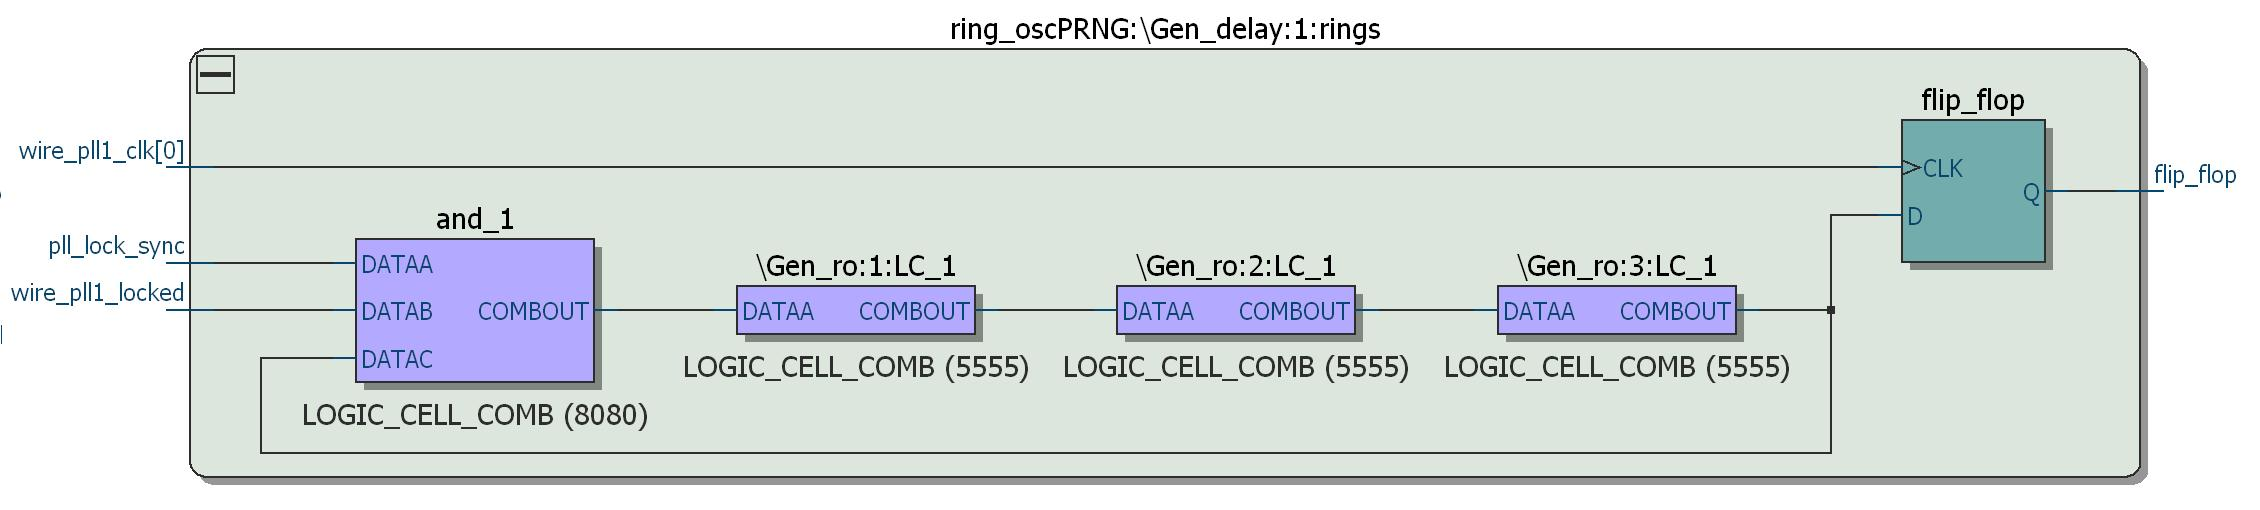
\includegraphics[ width=0.7\textwidth]{tech_map_viewer_post_mapping}
\caption{\textit{Technology map viewer} (post mapeo) de un ring con $3$ inversores.} \label{fig:postMap1ring}
\end{center}
\end{figure*}

Para lograr que cada {RO} tenga distintos comportamientos, cada uno debe ser ubicado en distintas posiciones del chip.
Para esto se lo debe asignar a una región previamente definida (\textit{LogicLock}).

La Figura \ref{fig:fpgaplan} muestra las $50$ regiones \emph{LogicLock}s utilizadas en este trabajo.
Se asigna un {RO} a cada región.
Las regiones se distribuyen sobre el chip para un análisis futuro de la importancia de la ubicación.
Cada región tiene $16$ {LAB}s, lo que permite aumentar el número de inversores de cada anillo.
%
\begin{figure*}
\begin{center}
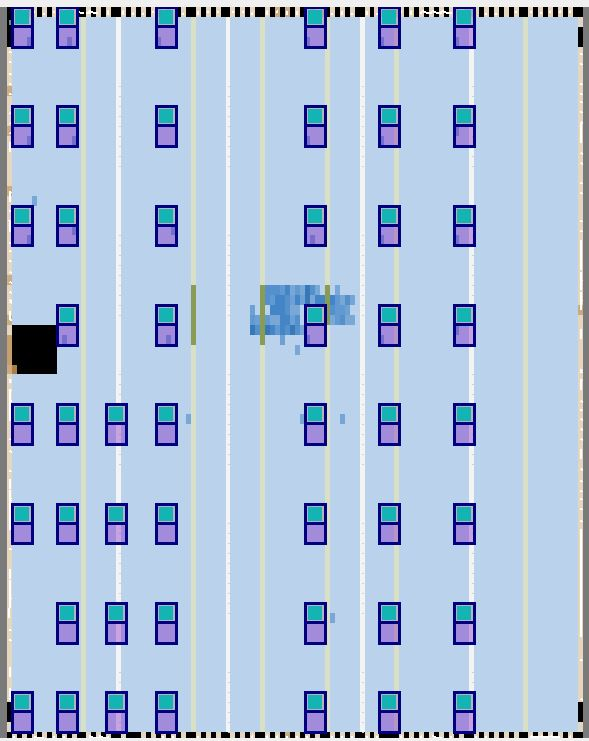
\includegraphics[ width=0.5\textwidth]{fpgaplan}
\caption{Vista de las regiones \emph{LogicLock} del \emph{Chip Planner}.}
\label{fig:fpgaplan}
\end{center}
\end{figure*}

Hay muchos factores que determinan la frecuencia de cada {RO}, y contribuyen a la imprevisibilidad de la salida:
\begin{enumerate}
\item Ubicación dentro de {LAB}: las diferentes ubicaciones entre los anillos pueden dar como resultado diferencias de tiempo.
\item Conexiones: incluso teniendo exactamente colocación idéntica de una {LUT} con respecto a otra en un anillo dado, no es posible tener exactamente el mismo {uso de recursos de enrutamiento} en las conexiones.
\item Selección de entrada: durante la etapa de enrutamiento, el \emph{fitter} elegirá qué entrada de la {LUT} se utiliza. Como el retraso a través de la {LUT} depende de cuál de las cuatro entradas se utiliza, los anillos tienen diferentes retardos.
\item Vecindad: incluso si os ROs pudieran ser exactamente identicos en los items anteriores, el retardo puede cambiar dependiendo de lo que se coloque y enrute alrededor del anillo.
\end{enumerate}


En la Figura \ref{fig:RTL3rings} (vista RTL) se muestra un {TRNG} usando $3$ {RO}s seguido por una compuerta XOR.
%
\begin{figure}
\begin{center}
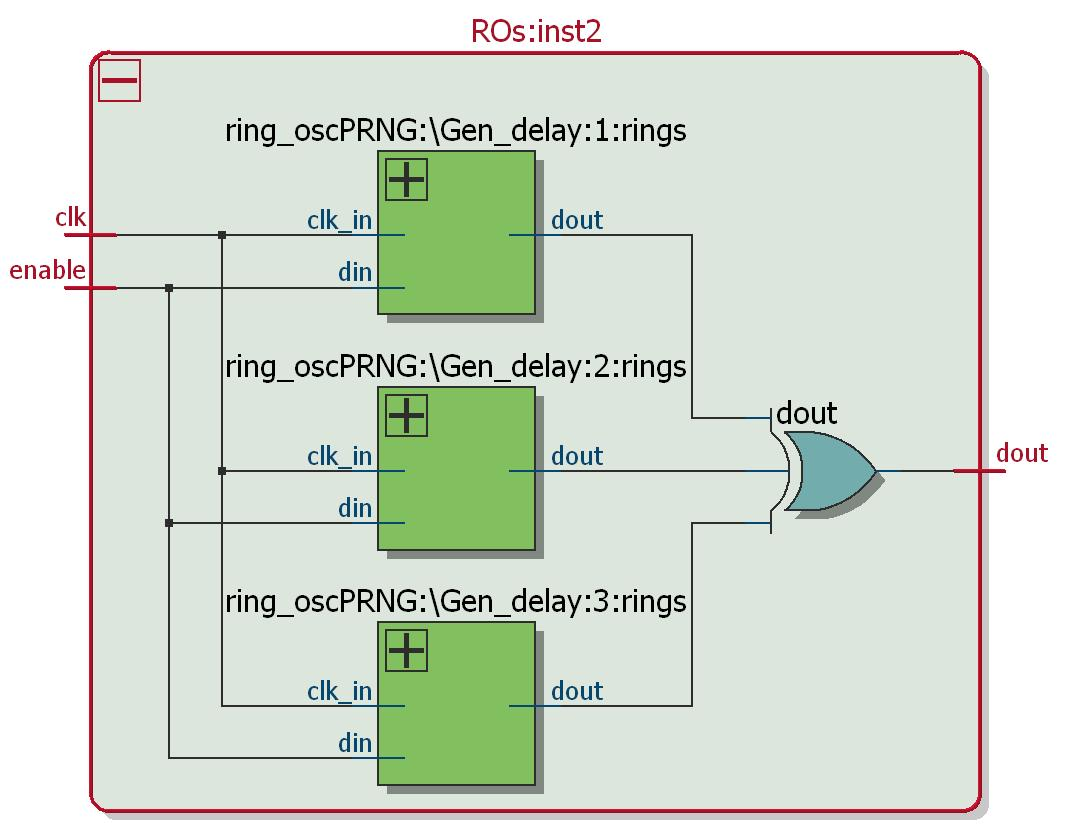
\includegraphics[ width=0.5\textwidth]{RTL_view_3ROs}
\caption{{RTL} de {TRNG} con $3$ {RO}s.}
\label{fig:RTL3rings}
\end{center}
\end{figure}

Para tener una idea de los recursos empleados para este diseño, la Tabla \ref{table:compilation} muestra el informe de compilación de un {TRNG} usando $15$ {RO}s cada uno con $3$ inversores.
\begin{table}
\begin{center}
\begin{tabular}{| l | c  c | }
	\hline
	\footnotesize{Elementos lógicos totales}         & $847/119,088$       & $( < 1 \%)$ \\ \hline
	\footnotesize{Funciones combinacionales totales} & $629/119,088$       & $( < 1 \%)$ \\ \hline
	\footnotesize{Registros lógicos dedicados}       & $617/119,088$       & $( < 1 \%)$ \\ \hline
	\footnotesize{Registros totales}                 & $617$               &             \\ \hline
	\footnotesize{Bits de memoria totales}           & $131,072/3,981,312$ & $( 3 \%)$   \\ \hline
\end{tabular}
\end{center}
\caption{Reporte de compilación de un {RO} basado en {TRNG}, utiliza $15$ {RO}s de $3$ inversores cada uno.}
\label{table:compilation}
\end{table}

\subsection{Resultados}
\label{sec:results}

La herramienta \emph{Embedded Logic Analyzer} se utilizó para recopilar las secuencias aleatorias generadas.
Esta es una {herramienta de depuración a nivel de sistema}, proporcionada por $ Altera $ \cite{QUARTUS}, que captura y almacena el comportamiento de la señal en tiempo real y permite observar las interacciones entre el hardware y el software en los diseños del sistema.
Después de adquirir los datos y guardarlos en un archivo {SignalTap II}, pueden ser analizado o visto como una forma de onda.
Este procedimiento no introduce \textit{jitter} ni distorsión en la señal medida.

Se utilizaron archivos de datos con $917504$bits cada uno para cada {TRNG}.
Consideramos conjuntos de $N_ {RO}$ anillos, cada uno con $3$ inversores; $N_{RO}=2$, $3$, $4$, $5$, $6$, $7$, $15$, $25$ y $50$.

Los datos de SignalTap se procesaron usando {Matlab}.
Se agruparon los datos en palabras de $6$ bits sin superposición, por lo que se generaron archivos con $152917$ datos cada uno.
Se calcularon los cuantificadores descriptos en la Sección \ref{capCuanti} para todos los archivos generados.

También se evaluaron otros generadores de ruido conocidos para comparar su calidad con la de los {TRNG} basados en {RO}.
Los ruidos analizados fueron:

\begin{itemize}
  \item Mersenne Twister pseudo-random number generator, \cite{Matsumoto1998}.
  \item Dos algoritmos empleados para generar datos aleatorios por \textit{Matlab} (método congruente multiplicativo) y Excel \cite{McLeod1985}.
  \item Dos {ruidos físicos}: ruido de decaimiento radiactivo \cite{Walker2001} y ruido atmosférico \cite{Haahr}.
  Los archivos de datos para estos ruidos están disponibles en los online en los sitios referidos.
  \item Dos mapas caóticos $M^1$ y sus versiones iteradas $M^2$ a $M^8$ \cite{DeMicco2008} para el mapa Logístico y el {Three Way Bernoulli Map} ({TWBM}).
\end{itemize}

La Figura \ref{fig:HBPvsHhis_all} muestra los resultados en el plano de doble entropía $H_ {BP} \times H_{hist}$ para todos los ruidos estudiados.
Puede verse que los ruidos físicos, el algoritmo \emph{Mersenne Twister} y los {PRNG}s utilizados en {Matlab}(función {rand}) y en {Excel} (función {RAND}), tienen el valor máximo para $H_{BP}$, lo que indica que todos los patrones de orden aparecen casi el mismo número de veces.
Sin embargo, estos cinco ruidos presentan un comportamiento muy diferente con respecto al cuantificador $H_{hist}$.
El {decaimiento radiactivo} es el peor, con $H_ {hist} \sim 0,5$, lo que indica que esta secuencia no muestra todos los valores posibles en la misma proporción.
Los números al lado de cada marcador para las secuencias caóticas indican el número de iteración.
Los mapas iterados tienen mayor $H_{BP}$ debido a su propiedad de mezcla \cite{DeMicco2008}.
El plano de entropía dual muestra que un aumento en el número de {RO}s mejora tanto $H_{BP}$ como $H_{hist}$.
%
\begin{figure*}
\begin{center}
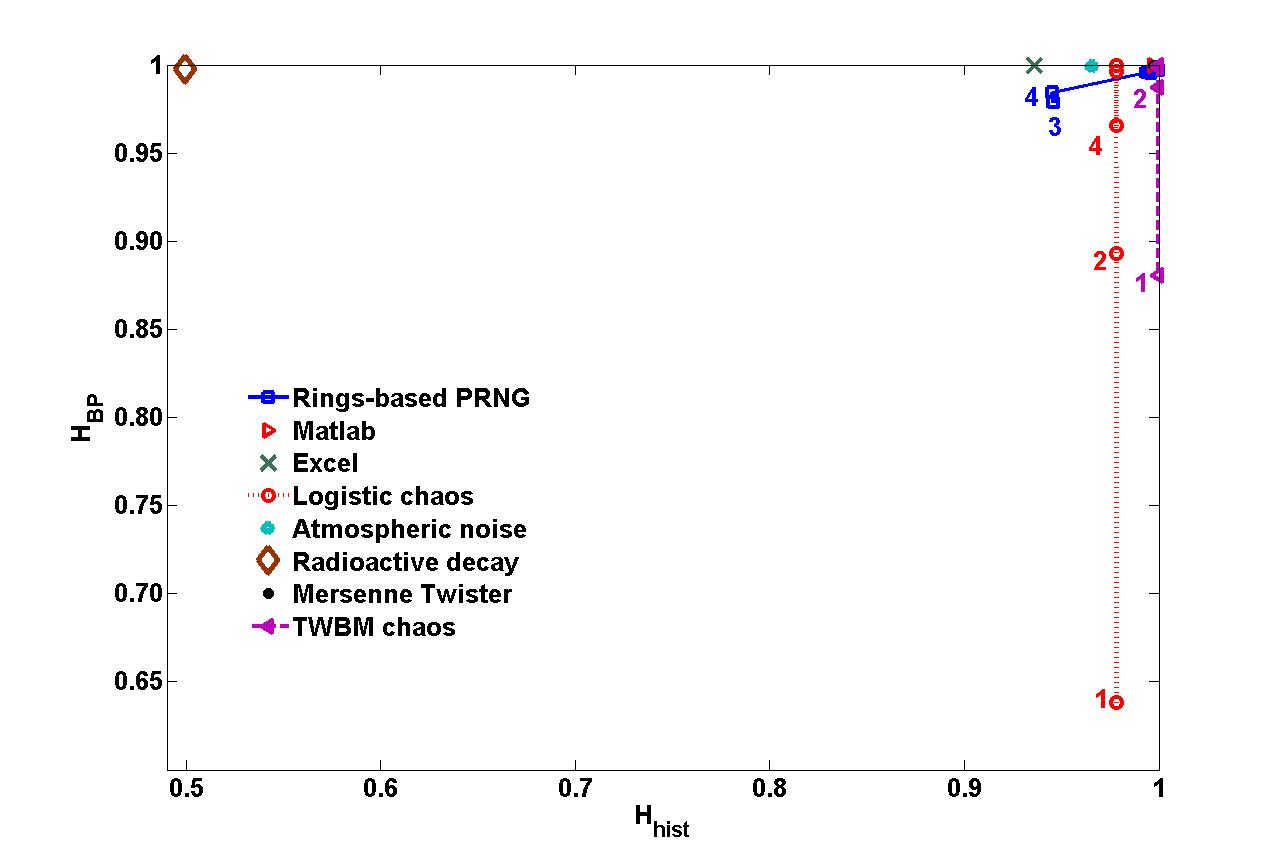
\includegraphics[ width=0.8\textwidth]{HhistvsHBP_t}
\caption{Plano $H_{hist} \times H_{BP}$ para distintos RNGs. Los números que siguen a cada cuadrado indica la cantidad de {RO}s utilizado en cada {TRNG}.
Los números al lado de cada punto en los resultados de los mapas {Logistico} y {TWBM} indican el número de iteración.}
\label{fig:HBPvsHhis_all}
\end{center}
\end{figure*}

La Figura \ref{HhistvsHBP_zoom} es una vista con más detalle de la Figura \ref{fig:HBPvsHhis_all} alrededor del punto ideal $(1,1)$.
Allí, se muestra la evolución de las secuencias cuando la cantidad de {RO}s aumenta de $5$ a $50$.
Se puede observar que a medida que el número de anillos aumenta los datos aumentan su mezcla y también el histograma tiende a ser más uniforme, por lo tanto, ambas propiedades mejoran.
Se puede determinar un umbral en el número de anillos, ya que los puntos saturan alrededor de $(0.997,1)$, por lo que este es el mejor {TRNG} posible, usar más de $15$ {RO}s no presenta ninguna mejora.
Como se dijo anteriormente, el cuantificador $H_ {hist}$ detecta la variación del histograma de la secuencia, y el cuantificador $ H_ {BP} $ refleja la mejora en la mezcla de datos.
Finalmente, las secuencias de Mersenne Twister y Matlab presentan un valor idéntico, ideal $H_ {BP}$ y un valor alto de $H_ {hist}$; no obstante, el histograma no es perfectamente uniforme (los valores no son equiprobables).
%
\begin{figure*}
	\begin{center}
		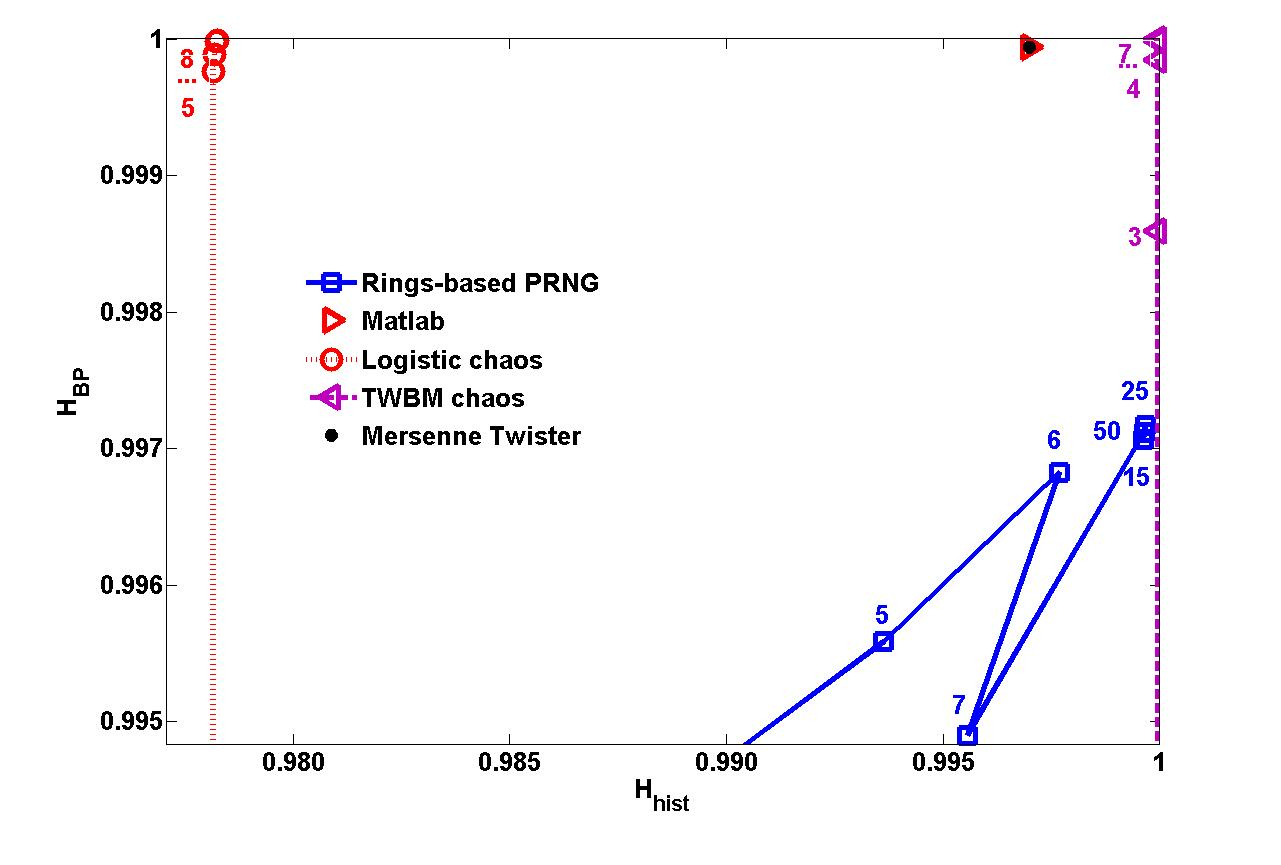
\includegraphics[ width=0.8\textwidth]{HhistvsHBP_z}
		\caption{Detalle de la Fig. \ref{fig:HBPvsHhis_all} alrededor del punto ideal $(1,1)$.}
		\label{HhistvsHBP_zoom}
	\end{center}
\end{figure*}